\documentclass{beamer}
\usetheme{metropolis} % Use metropolis theme

\title{ECON 3818: Introduction to Statistics with Computer Applications}
%\subtitle
\date{\today}
\author{Kyle Butts}

\definecolor{blue}{RGB}{0,114,178}
\definecolor{red}{HTML}{EB0E09}
\definecolor{yellow}{RGB}{240,228,66}
\definecolor{green}{RGB}{0,158,115}
\definecolor{maroon}{HTML}{AF3335}
\definecolor{purple}{HTML}{7E90B8}
\definecolor{buff-gold}{HTML}{CFB87C}
\definecolor{buff-grey}{HTML}{565A5C}
\definecolor{buff-lightgrey}{HTML}{A2A4A3}
\definecolor{buff-black}{HTML}{000000}


\definecolor{mybackground}{HTML}{ECECEC}
\setbeamercolor{background canvas}{bg= mybackground}
\setbeamercolor{alerted text}{fg=buff-gold!80!black}
\setbeamercolor{frametitle}{bg=buff-black}
\setbeamercolor{title}{fg=buff-grey}
\setbeamercolor{button}{bg=buff-gold}

% Allow to remove indent w/ \begin{itemize}[leftmargin= *]
\usepackage{enumitem}
\setlist[itemize]{label= \textbullet}

% \usepackage[libertine]{newtxmath}
\usepackage{longtable}
\usepackage{booktabs}
\usepackage{enumitem}

% \diagbox
\usepackage{diagbox}


\begin{document}

% Title Page ---------------------------------------
\maketitle

% Chapter 4 ----------------------------------------
\section{Chapter 4: Correlation}

\begin{frame}{Multiple Variables}
	Almost everything we've done so far has been \textit{univariate} statistics, but often we're interested in how multiple random variables are related?
	\begin{itemize}
		\item How does education affect earnings?
		\item How does race affect earnings?
		\item How does experience affect earnings?
	\end{itemize}
	
	Many events are \textit{dependent} on other random variables. In this chapter we'll formalize this concept.
\end{frame}

\begin{frame}{Probability Theory}
	Recall that with single random variables we characterized probabilities with
	\begin{itemize}
		\item PMF (probability mass function), $P(X=x)$, in discrete case
		\item PDF (probability density function), $f(x)$, in continuous case
	\end{itemize}
	
	When we have multiple random variables we use the \alert{joint distribution}
	\begin{itemize}
		\item $P(X=x, Y=y)$ in the discrete case
		\item $f(x,y)$ in the continuous case
	\end{itemize}
\end{frame}

\begin{frame}{Properties for Joint Distribution}
	For short hand, $P(x,y)=P(X=x, Y=y)$
	
	In this class we'll focus solely on the discrete case
	\begin{itemize}
		\item $0 \leq P(x,y) \leq 1$
		\item $\sum_x \sum_y P(x,y)=1$
	\end{itemize}
	
	As long as X and Y are \alert{not independent}
	$$P(x,y) \neq P(x)P(y)$$
\end{frame}


\begin{frame}{Example}
	Suppose that $X$ is the number of girls born out of three kids and $Y$ is whether the first child is a girl.
	\begin{center}
		\begin{tabular}{|l|l|l|}
			\hline
			Outcome & $X$ & $Y$ \\
			\hline
			BBB     & 0   & 0   \\
			\hline
			GBB     & 1   & 1   \\
			\hline
			BGB     & 1   & 0   \\
			\hline
			BBG     & 1   & 0   \\
			\hline
			GGB     & 2   & 1   \\
			\hline
			GBG     & 2   & 1   \\
			\hline
			BGG     & 2   & 0   \\
			\hline
			GGG     & 3   & 1   \\
			\hline
		\end{tabular}
	\end{center}
\end{frame}

\begin{frame}{Example}
	Notice that the sample spaces are $S_X =\{0,1,2,3\}$ and $S_Y=\{0,1\}$. The associated joint probabilities are:
	\begin{center}
		\begin{tabular}{|c|c|c|}
			\hline
			\diagbox{$X$}{$Y$} & 0   & 1   \\
			\hline
			0                            & 1/8 & 0   \\
			\hline
			1                            & 2/8 & 1/8 \\
			\hline
			2                            & 1/8 & 2/8 \\
			\hline
			3                            & 0   & 1/8 \\
			\hline
		\end{tabular}
	\end{center}
\end{frame}

\begin{frame}{Example}
	Let's check this table satisfies the definition of a joint distribution
	\begin{itemize}
		\item $0 \leq P(x,y) \leq 1 \checkmark$
		\item $\sum_x \sum_y P(x,y)=1$
	\end{itemize}
	\begin{align*}
		\sum_{x\in S_X}\sum_{y\in S_Y}Pr(x,y) = & Pr(0,0) + Pr(0,1) + Pr(1,0) + Pr(1,1)   \\
		& + Pr(2,0) + Pr(2,1) + Pr(3,0) + Pr(3,1) \\
		& = 1/8 + 0 + 2/8 + 1/8 \\
		& +1/8 + 2/8 + 0 + 1/8 = 1 \checkmark     
	\end{align*}
\end{frame}

\begin{frame}{Clicker Question}
	Given the following joint probability mass function, what is the probability of the NASDAQ increasing in value and your portfolio loses value?
	\begin{columns}
		\begin{column}{.8\textwidth}
			\begin{center}
				\begin{tabular}{ |c|c|c| }
					\hline
					\diagbox{NASDAQ}{Portfolio} & Increases & Decreases \\
					\hline
					Increases                        & 0.40      & .05       \\
					\hline
					Decreases                        & .15       & 0.40      \\
					\hline
				\end{tabular}
			\end{center}
		\end{column}
		\begin{column}{0.3\textwidth}
			\begin{enumerate}[label=(\alph*)]
				\item 0.40
				\item 0.05
				\item 0.15
				\item 0.45
			\end{enumerate}
		\end{column}
	\end{columns}
\end{frame}

\begin{frame}{Clicker Question}
	Given the following joint probability mass function, what is the probability that the NASDAQ increases in value?
	\begin{columns}
		\begin{column}{.8\textwidth}
			\begin{center}
				\begin{tabular}{ |c|c|c| }
					\hline
					\diagbox{NASDAQ}{Portfolio} & Increases & Decreases \\
					\hline
					Increases                        & 0.40      & .05       \\
					\hline
					Decreases                        & .15       & 0.40      \\
					\hline
				\end{tabular}
			\end{center}
		\end{column}

		\begin{column}{0.3\textwidth}
			\begin{enumerate}[label=(\alph*)]
				\item 0.40
				\item 0.05
				\item 0.15
				\item 0.45
			\end{enumerate}
		\end{column}
	\end{columns}
\end{frame}

\begin{frame}{Clicker Question}
	Given the following joint probability mass function, what is the probability that the NASDAQ increases in value, conditional on the portfolio value decreases?
	\begin{columns}
		\begin{column}{.8\textwidth}
			\begin{center}
				\begin{tabular}{ |c|c|c| }
					\hline
					\diagbox{NASDAQ}{Portfolio} & Increases & Decreases \\
					\hline
					Increases                        & 0.40      & .05       \\
					\hline
					Decreases                        & .15       & 0.40      \\
					\hline
				\end{tabular}
			\end{center}
		\end{column}

		\begin{column}{0.3\textwidth}
			\begin{enumerate}[label=(\alph*)]
				\item 0.111
				\item 0.889
				\item 0.05
				\item 0.40
			\end{enumerate}
		\end{column}
	\end{columns}
\end{frame}

\frame

\begin{frame}{Visualizing a Joint Distribution}
	The most useful 
	for displaying the relationship between two \underline{quantitative} variables is a \alert{scatterplot}
	\begin{itemize}
		\item Shows relationship between two quantitative variables
		      \begin{itemize}
		      	\item Each axis represents a variable
		      	\item Individual data appear as a point, fixed by the values of both variables
		      \end{itemize}
	\end{itemize}
\end{frame}

\begin{frame}{Scatterplot Example}
	\begin{center}
		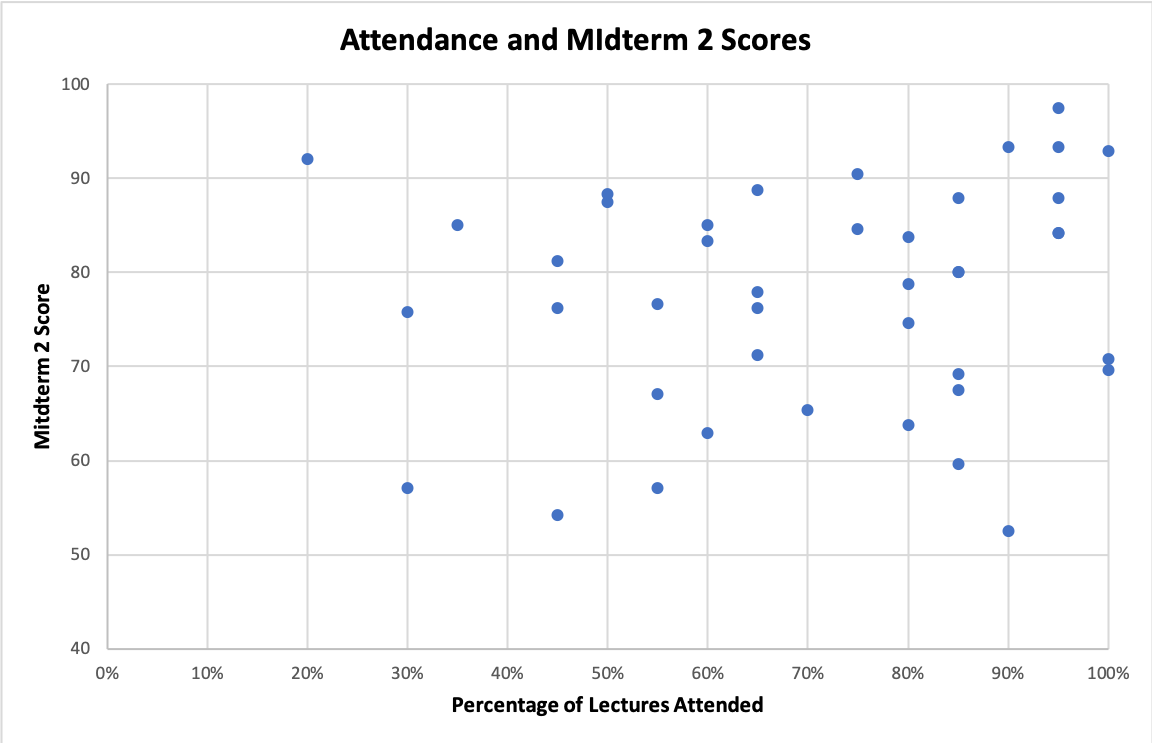
\includegraphics[width=0.8\textwidth]{midtermscatter}
	\end{center}
\end{frame}

\begin{frame}{Interpreting a Scatterplot}
	\begin{itemize}
		\item Looking for patterns, and deviations from that pattern
		      \begin{itemize}
		      	\item Direction, form, strength of relationship
		      	\item Any outliers?
		      \end{itemize}
		\item Describing the association
		      \begin{itemize}
		      	\item \alert{Positive Association}: above-average values of one tend to accompany above-average values of the other, and below-average values also tend to occur together
		      	\item \alert{Negative Association}: above-average values of one tend to accompany below-average values of the other, and vice versa
		      \end{itemize}
		\item In general, if one variable is explanatory (influences change) and one is a response variable (outcome), then the explanatory variable is plotted on the x-axis
	\end{itemize}
\end{frame}

\begin{frame}{Correlation}
	We need to supplement the graph with a numerical measure, generally we use \alert{correlation}.
	
	
	
	\begin{definition}[Correlation]
		The correlation measures the direction and strength of the linear relationship between two quantitive variables. Correlation is usually written as $r$
	\end{definition}
\end{frame}

\begin{frame}{Covariance}
	In order to understand correlations, we must first discuss \alert{covariance}
	
	Recall: $V(aX+bY)=a^2V(X)+b^2V(Y)+2ab\cdot cov(X,Y)$
	
	Covariance measures the joint variability of two random variables
	\small{\begin{itemize}
		\item Sign of covariance explains direction of relationship
		\item Magnitude of covariance is hard to interpret -- hence the usage of \alert{correlation coefficient}
		\item Covariance equals zero whenever X and Y are \alert{independent}
		\end{itemize}}
\end{frame}

\begin{frame}{Covariance}
	We use the following formula to calculate covariance
	$$cov(X,Y)=E(XY)-E(X)E(Y)$$
	Note: $E(XY) \neq E(X)E(Y)$ unless X \& Y are independent and then cov(X,Y)=0
	
	
	The magnitude of covariance depends on the units of X \& Y
	\begin{itemize}
		\item This means $cov(A,B) > cov(C,D)$ \alert{does not} imply that A\&B have stronger relationship than C\&D
		\item In order to compare relationships we must find a way to normalize their covariances 
	\end{itemize}
\end{frame}

\begin{frame}{Correlation}
	\begin{definition}[Correlation]
		The correlation measures the direction and strength of the linear relationship between two quantitive variables. Correlation is usually written as $r$
	\end{definition}
	To calculate correlation, we normalize the covariance as so:
	$$r=\frac{cov(X,Y)}{\sqrt{V(X)}\cdot \sqrt{V(Y)}}$$
\end{frame}

\begin{frame}{Correlation}
	Notes on correlation
	\begin{itemize}
		\item Values are always between -1 and 1
		      \begin{itemize}
		      	\item $1 \rightarrow$ perfectly linear positive relationship (variables move same direction and same magnitude)
		      	\item $-1 \rightarrow$ pefectly linear negative relationship (variables move in opposite direction but same magnitude) 
		      \end{itemize}
		\item Correlations are unit-less
		\item \small{\alert{Doesn't imply a causal relationship}}
	\end{itemize}
	Drawbacks of correlation
	\begin{itemize}
		\item Only measures \textit{linear relationships}
		      \begin{itemize} 
		      	\item Just because correlation is zero doesn't necessarily mean variables are independent
		      \end{itemize}
		\item Not resistant to outliers
	\end{itemize}
\end{frame}

\begin{frame}{Correlations - Visualized}
	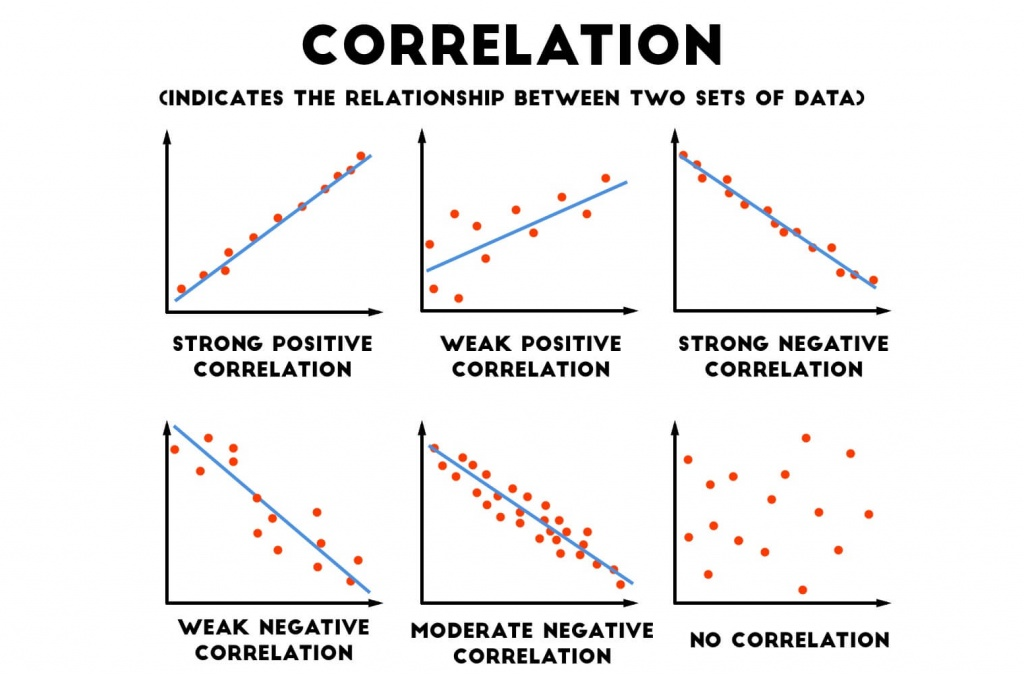
\includegraphics[width=\textwidth]{correlations.jpg}
\end{frame}

\begin{frame}{Why Correlation isn't Perfect}
	\begin{center}
		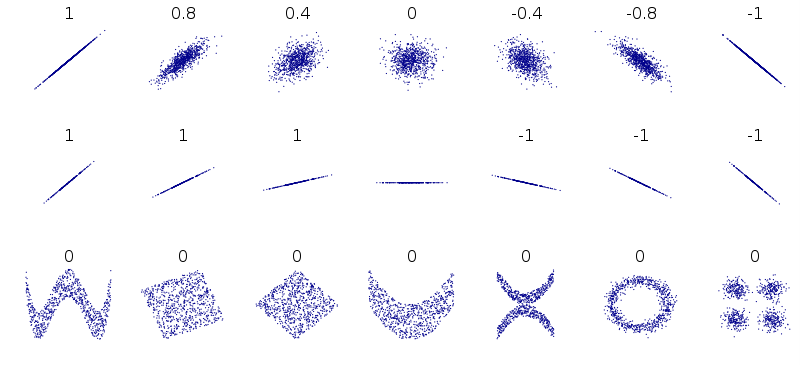
\includegraphics[width=\textwidth]{corr}
	\end{center}
\end{frame}

\begin{frame}{Covariance and Independence}
	Since covariance (and correlations) only measure linear relationships:
	$$cov(X,Y) = 0 \nrightarrow X \& Y \text{ are independent}$$
	
	However, since $E(XY)=E(X)E(Y)$ when X \& Y are independent:
	$$X \& Y \text{ are independent} \rightarrow cov(X,Y)=0$$
\end{frame}


\begin{frame}{Joint Distributions}
	When calculating the covariance we use equation $cov(X,Y) = E(XY)-E(X)E(Y)$
	\begin{center}
		\small{\begin{tabular}{|c|c|c|}
			\hline
			\diagbox{$X$}{$Y$} & 0 & 1 \\
			\hline
			0 & 1/8 & 0 \\
			\hline
			1 & 2/8 & 1/8 \\
			\hline
			2 & 1/8 & 2/8 \\
			\hline
			3 & 0 & 1/8 \\
			\hline
			\end{tabular}}
	\end{center}
	$$E(XY)=x\cdot y \cdot P(x,y)$$
	In this example:
	$$E(XY)=(0\cdot 0 \cdot 1/8) + (0\cdot  1\cdot 0) + (1\cdot 0 \cdot 2/8) + (1\cdot 1 \cdot 1/8)+$$
	$$(2\cdot 0 \cdot 1/8) + (2\cdot 1 \cdot 2/8) + (3\cdot 0 \cdot 0) + (3\cdot 1 \cdot 1/8)=1$$
\end{frame}

\begin{frame}{Marginal Probabilties}
	In order to calculate $E(X)$ and $E(Y)$ from a joint distribution we must first calculate the \alert{marginal probabilities} of both X and Y. 
	\begin{center}
		\begin{tabular}{|c|c|c|c|}
			\hline
			\diagbox{$X$}{$Y$} & 0   & 1   & $Pr(X)$ \\
			\hline
			0                       & 1/8 & 0   & 1/8     \\
			\hline
			1                       & 2/8 & 1/8 & 3/8     \\
			\hline
			2                       & 1/8 & 2/8 & 3/8     \\
			\hline
			3                       & 0   & 1/8 & 1/8     \\
			\hline
			$Pr(Y)$                 & 4/8 & 4/8 & 1       \\
			\hline
		\end{tabular}
	\end{center}
	These marginal probabilities, $P(X=x) $are calculated adding up the probabilities across each scenario where $X=x$
\end{frame}

\begin{frame}{Marginal Probabilities}
	We can use these marginal probabilities to calculate $E(X)$ and $E(Y)$.
	\begin{center}
		\begin{tabular}{|c|c|c|c|}
			\hline
			\diagbox{$X$}{$Y$} & 0   & 1   & $Pr(X)$ \\
			\hline
			0                       & 1/8 & 0   & 1/8     \\
			\hline
			1                       & 2/8 & 1/8 & 3/8     \\
			\hline
			2                       & 1/8 & 2/8 & 3/8     \\
			\hline
			3                       & 0   & 1/8 & 1/8     \\
			\hline
			$Pr(Y)$                 & 4/8 & 4/8 & 1       \\
			\hline
		\end{tabular}
	\end{center}
	$E(X)=(0 \cdot 1/8) + (1 \cdot 3/8) + (2 \cdot 3/8) + (3 \cdot 1/8) =1.5$
	$E(Y)=(0 \cdot 4/8) + (1 \cdot 4/8) =0.5$
\end{frame}

\begin{frame}{Covariance of Joint Distribution}
	All of that work leads us here:
	$$E(XY)=1$$
	$$E(X)= 1.5 $$
	$$E(Y)= 0.5$$
	$$cov(X,Y)=E(XY)-E(X)E(Y) =1 - (1.5 \cdot 0.5) = 0.25$$
\end{frame}

\begin{frame}{Covariance to Correlation}
	Again, we often use correlation instead of covariance because correlation \alert{does not depend on the units}
	
	To find correlation from covariance we use the following equation:
	$$r = \frac{\text{cov(X,Y)}}{\sqrt{\text{V(X)}\cdot \text{V(Y)}}}$$
	So we need to calculate the variance of X and Y, using information about the joint probabilities
\end{frame}

\begin{frame}{Covariance to Correlation}
	Recall the joint probabilities we gathered from the table
	\begin{center}
		\begin{tabular}{c|ccc|c}
			X & P(X) &   & Y & P(Y) \\
			\hline
			0 & 1/8  &   & 0 & 4/8  \\
			1 & 3/8  &   & 1 & 4/8  \\
			2 & 3/8  &   &   &      \\
			3 & 1/8  &   &   &      \\
		\end{tabular}
	\end{center}
	
	$ E(X^2) = (0^2 \cdot 1/8) + (1^2 \cdot 3/8) + (2^2 \cdot 3/8) + (3^2 \cdot 1/8) =3$ \\
	
	$ E(Y^2)=(0^2 \cdot 4/8) + (1^2 \cdot 4/8) =0.5$
	
\end{frame}

\begin{frame}{Covariance to Correlation}
	$E(X)=1.5$ and $E(X^2)=3 \rightarrow V(X)=3-1.5^2= 0.75$
	
	$E(Y)=0.5$ and $E(Y^2)=0.5 \rightarrow V(Y)=0.5-0.5^2 = 0.25$
	
	$cov(X,Y)=0.25$
	
	$$r = \frac{\text{cov(X,Y)}}{\sqrt{\text{V(X)}}\cdot \sqrt{\text{V(Y)}}} =\frac{0.25}{\sqrt{0.75}\cdot\sqrt{0.25}}=0.577$$
\end{frame}

\begin{frame}{Clicker Question}
	What can be said of the correlation between the brand of an automobile and its quality?
	\begin{enumerate}[label=(\alph*)]
		\item The correlation is negative, because smaller cars tend to have higher quality and larger cars tend to have lower quality.
		\item The correlation is positive, because better brands have higher quality.
		\item If the correlation is negative, an arithmetic mistake was made; correlation must be positive.
		\item Correlation makes no sense here, because brand is a categorical variable. %
	\end{enumerate}
\end{frame}

\begin{frame}{Clicker Question}
	Which of the following statements is false?
	\begin{enumerate}[label=(\alph*)]
		\item Older men tend to have lower muscle density, so the correlation between age and muscle density in older men must be negative.
		\item Older children tend to be taller than younger children, so the correlation between age and height in children must be positive.
		\item A researcher finds that the correlation between two variables is close to 0, so the two variables must be unrelated.%
		\item Taller people tend to be heavier than shorter people, so the correlation between height and weight must be positive.
	\end{enumerate}
\end{frame}


\end{document}